\documentclass{standalone}
\usepackage{tikz}
\usetikzlibrary{positioning,shapes.geometric,arrows}
\begin{document}
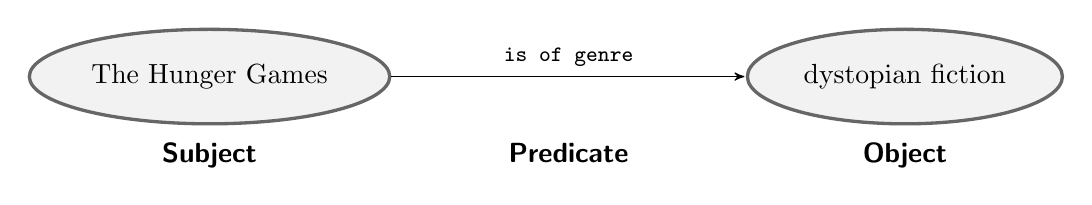
\begin{tikzpicture}[
        vertex/.style={
                ellipse,
                draw=black!60,
                fill=black!5,
                very thick,
                minimum width = 4cm,
                minimum height = 1.2cm
            },
        predicate/.style = {font=\footnotesize\ttfamily},
        >= stealth',
        shorten >= 0.5pt
    ]
    \node[vertex,label={[yshift=-1.9cm,font=\sffamily\bfseries]Subject}] (thg) {The Hunger Games};
    \node[vertex,label={[yshift=-1.9cm,font=\sffamily\bfseries]Object}] (dystopian) [right=4.5cm of thg] {dystopian fiction};

    \path[->] (thg) edge node[predicate,above,label={[yshift=-1.7cm,font=\sffamily\bfseries]Predicate}] {is of genre} (dystopian);
\end{tikzpicture}
\end{document}